\section{Laboratory work implementation}

\subsection{Tasks and Points}
\begin{itemize}
\item \textbf{Basic Level (grade 5 - 6) you should be able to:}
	\begin{enumerate}
	\item Create a Windows application what will dispaly a dialog box on some event (ex. on clicking some button)
      \item Add a system menu to your application with at least 3 items (add actions to that items)
      \item Hook keyboard input. Add 2 custom events for 2 different keyboard combinations (ex. change window background on ctrl+space)
      \end{enumerate}
\item \textbf{Normal Level (grade 7 - 8) you should be able to:}
      \begin{enumerate}
    \item Realize the tasks from \textit{Basic Level}.
    \item Add a scroll bar that will change any visible parameter of any other element (color of a text) OR other 2 scroll bars that will manage main window size or position
          \end{enumerate}
\item \textbf{Advanced Level (grade 9 - 10) you should be able to:}
      \begin{enumerate}
    \item Realize the tasks from \textit{Normal Level}.
    \item Customize your application by adding an icon and using different cursor in application
    \item Add a listbox and attach some events when any element is accessed (clicked)
          \end{enumerate}
\item \textbf{for Bonus Point Tasks :}
\begin{enumerate}
	\item Use a scroll bar to scroll through application working space. Scroll should appear only when necessary (eg. when window width is smaller than 300px)
    \end{enumerate}
  \end{itemize}  


\subsection{Prove your work with screens}

\begin{figure}[h!]
  \centering
    {%
      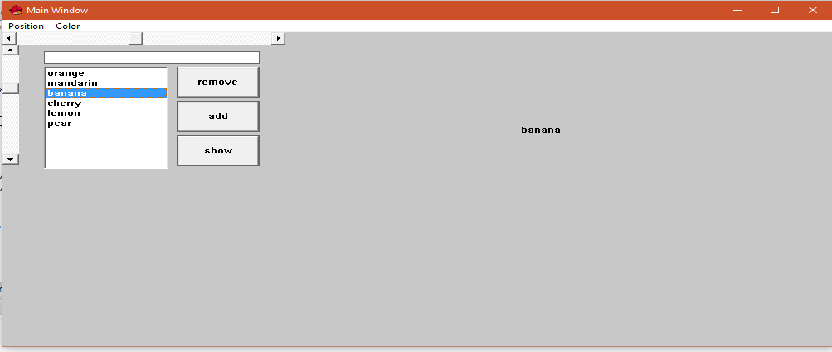
\includegraphics[width=0.5\textwidth]{1}}
  \caption{Add/Rmv/Show elemets to list and select one to display in the right part of window.}
\end{figure}

\begin{figure}[h!]
  \centering
    {%
      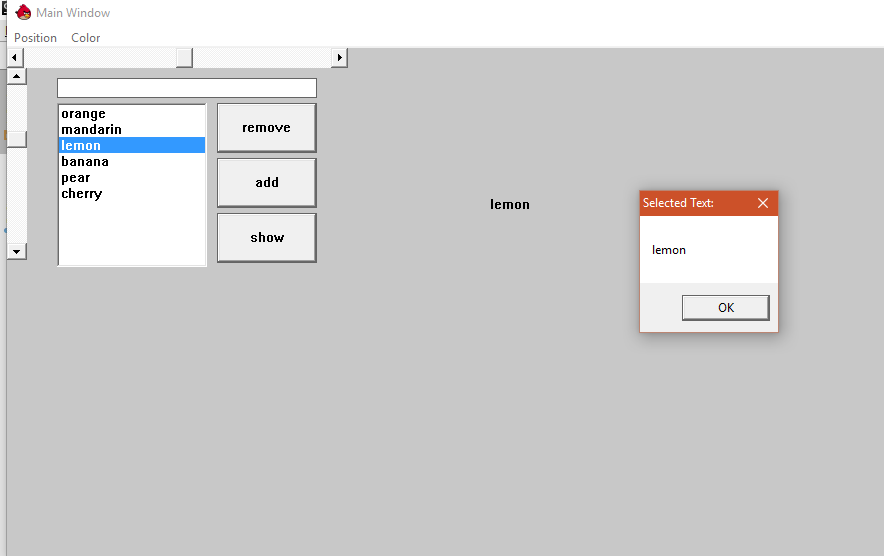
\includegraphics[width=0.5\textwidth]{2}}
  \caption{Click show button to pop up the name of selected element}
\end{figure}

\begin{figure}[h!]
  \centering
    {%
      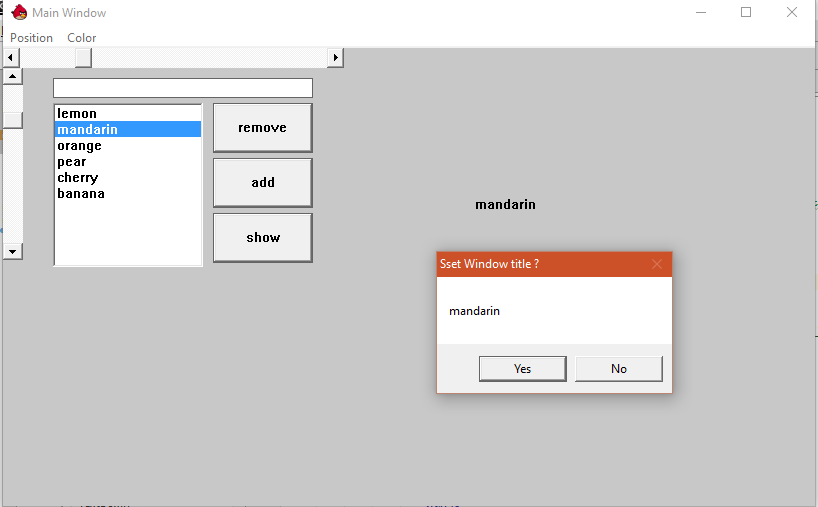
\includegraphics[width=0.5\textwidth]{3}}
  \caption{Double click on an element from the list to set it as window title}
\end{figure}

\begin{figure}[h!]
  \centering
    {%
      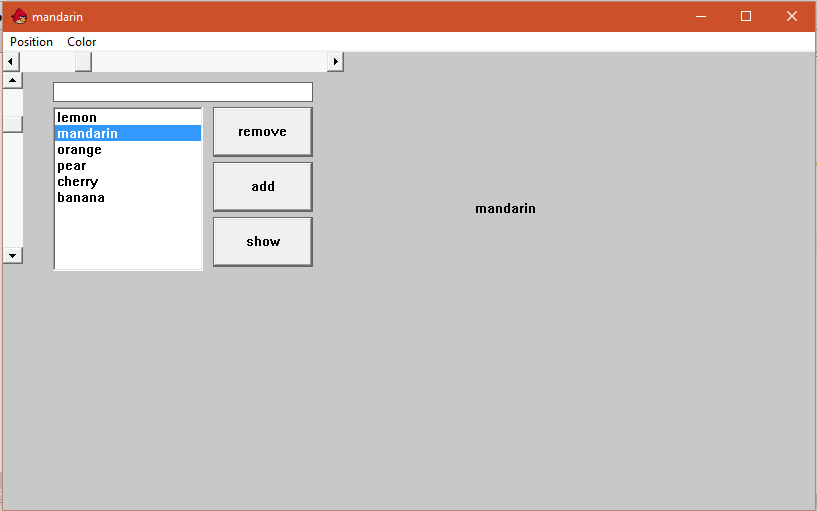
\includegraphics[width=0.5\textwidth]{4}}
  \caption{For example double click mandarin press ok and see mandarin title}
\end{figure}

\begin{figure}[h!]
  \centering
    {%
      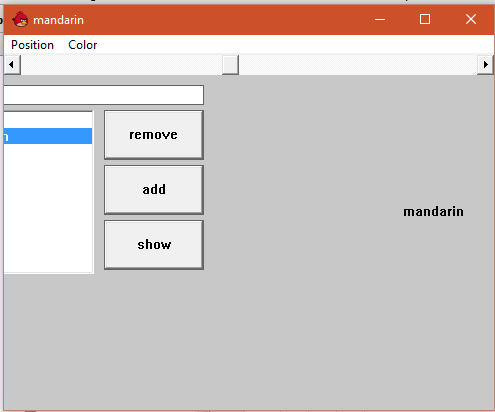
\includegraphics[width=0.5\textwidth]{5}}
  \caption{Resize the window and move the scroll to see all content }
\end{figure}
\begin{figure}[h!]
  \centering
    {%
      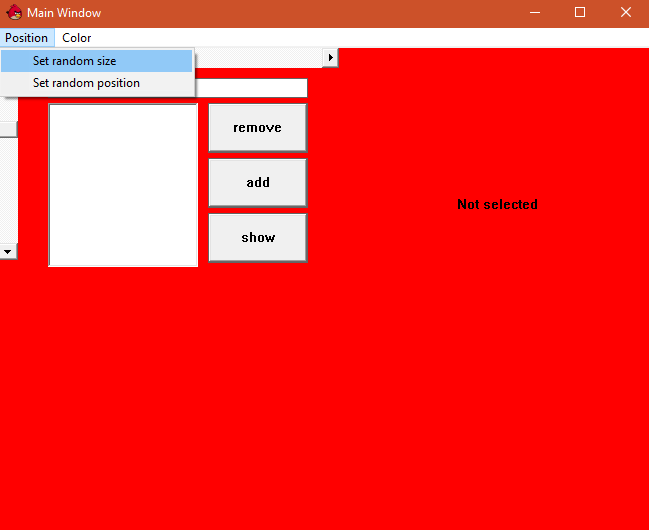
\includegraphics[width=0.5\textwidth]{7}}
  \caption{Chose from window menu set random size to set random size }
\end{figure}
\begin{figure}[h!]
  \centering
    {%
      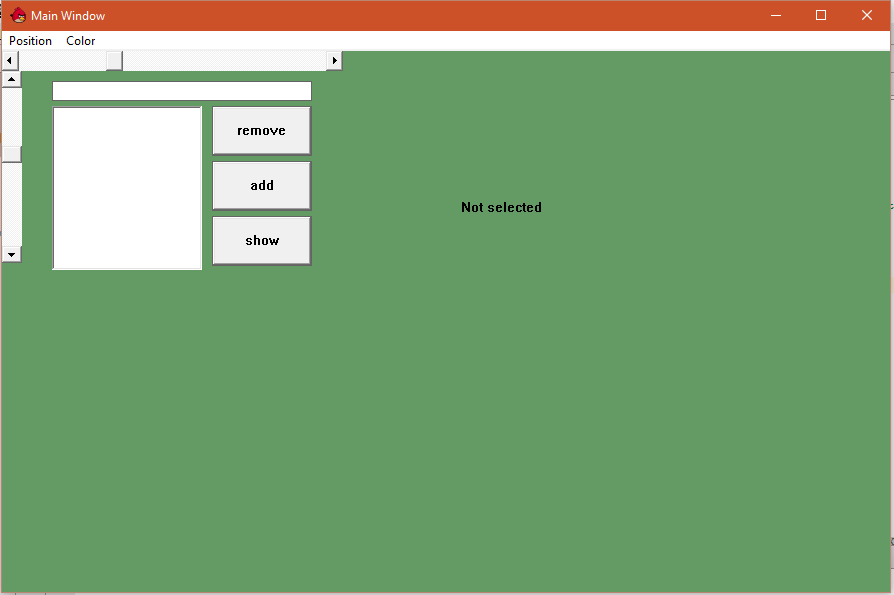
\includegraphics[width=0.5\textwidth]{8}}
  \caption{Chose from window menu set position size to set random position }
\end{figure}
\begin{figure}[h!]
  \centering
    {%
      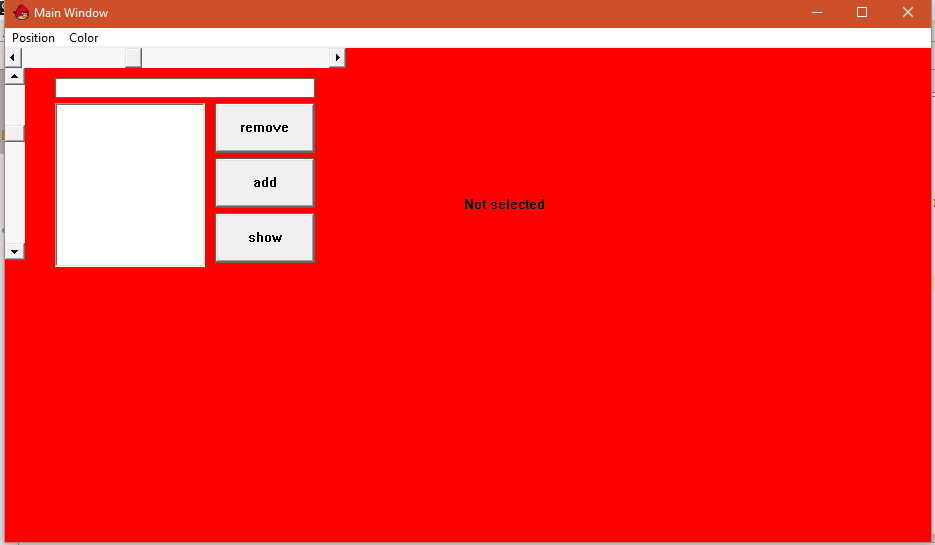
\includegraphics[width=0.5\textwidth]{6}}
  \caption{Press ctrl+C to change window color  also press ctrl+V to close window}
\end{figure}
\clearpage